\documentclass[handout]{beamer}
\usepackage{array}
\usepackage{german}
\usepackage{graphicx}
\usepackage[utf8]{inputenc}
\usepackage[T1]{fontenc}
\mode<beamer>{%
\usetheme{Copenhagen}
}
\usepackage[orientation=landscape,size=a3,debug,scale=2.7]{beamerposter}
\title[]{}
\begin{document}
\begin{frame}
\frametitle{%\hspace{0pt plus 1 filll}
MathSem 2022: Spezielle Funktionen}
\begin{columns}[onlytextwidth]
\begin{column}{0.31\textwidth}
%{%\bf
%\large Das Buch zum Seminar}
%\bigskip
%\vskip 1cm
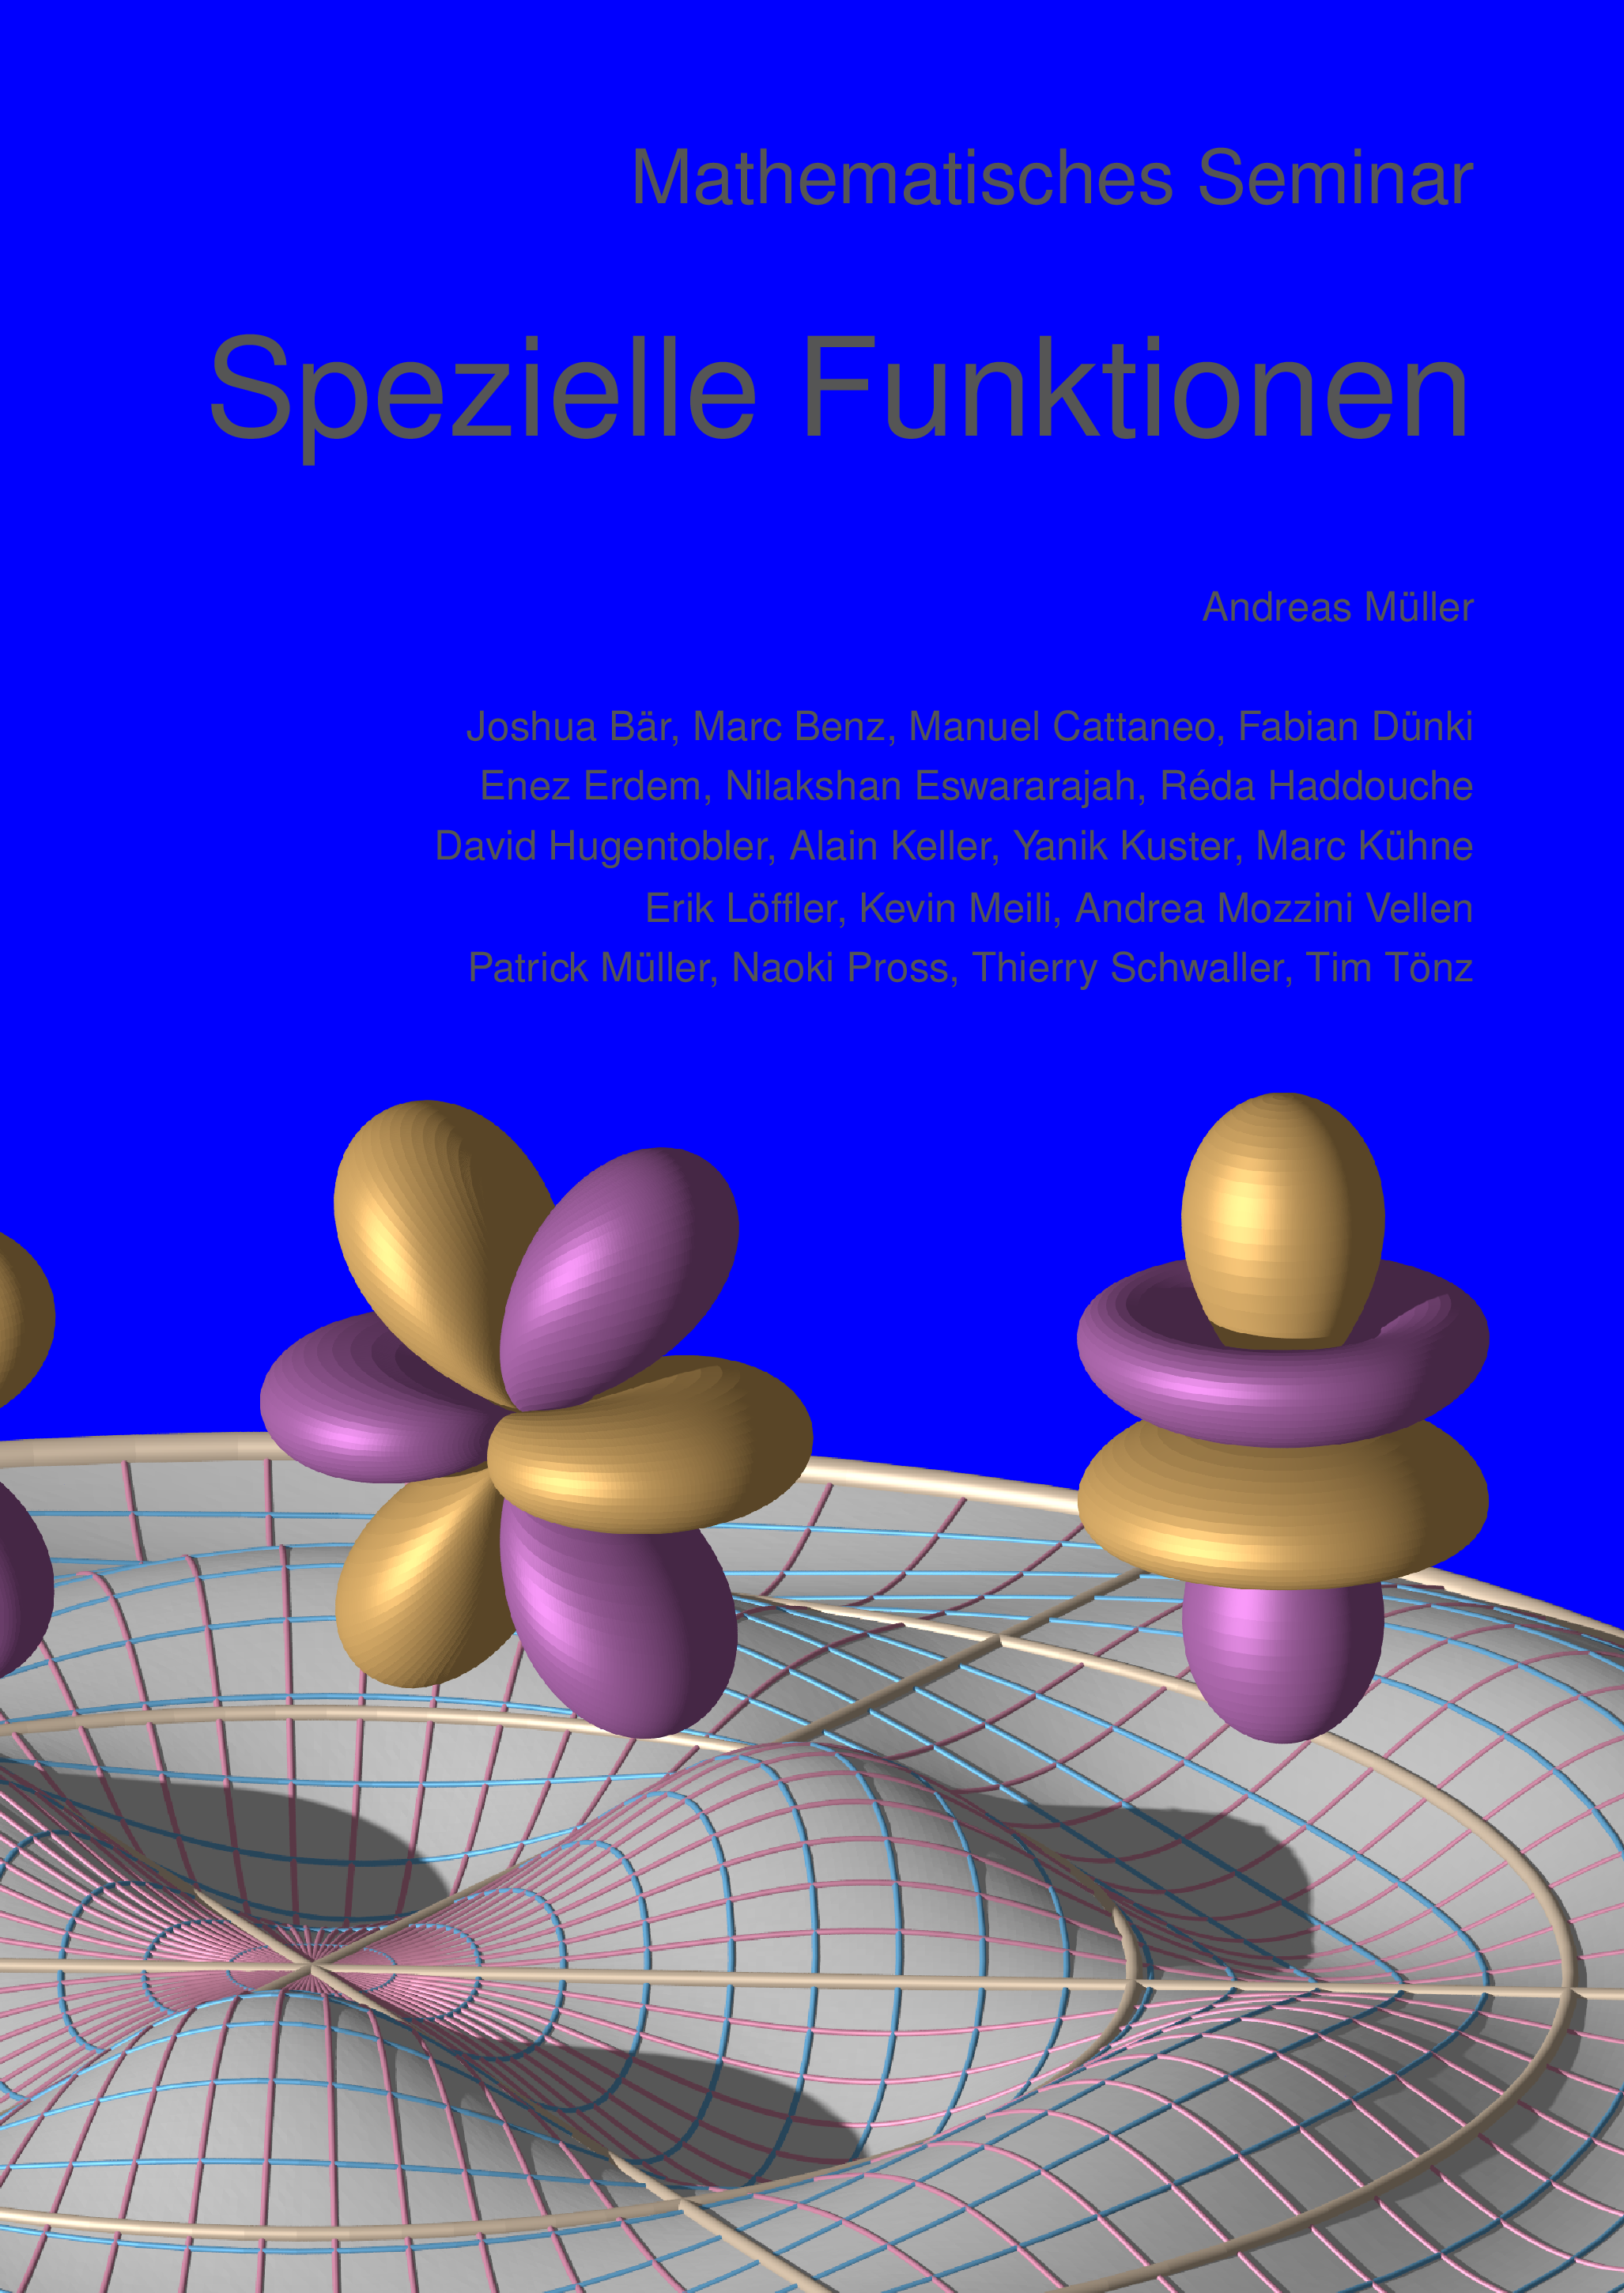
\includegraphics[width=\hsize]{../cover/buchcover.png}
\vskip 0.2cm
\bigskip
\bigskip
Erscheint im Herbst 2022.
Anfragen an
Prof.~Dr.~Andreas Müller,
{\texttt{andreas.mueller@ost.ch}}
\bigskip
\bigskip
\bigskip
%\vskip 1.2cm
\end{column}
\begin{column}{0.67\textwidth}
\begin{description}
\item[Teil 1:] Grundlagen
\begin{enumerate}
\item Sampling und Geometrie
\item Frames
\item Fouriertheorie und die $L^2$-Hilberträume
\item Das Haar-Wavelet
\item Stetige Wavelettransformation
\item Multiskalenanalyse
\item Waveletanalyse und Waveletsynthese als Faltungsfilter
\item Wavelets mit kompaktem Träger
\item Spline-Wavelets
\end{enumerate}
\item[Teil 2:] Anwendungen und weiterführende Themen
\begin{enumerate}
\setcounter{enumi}{9}
\end{enumerate}
\end{description}
\end{column}
\end{columns}
\end{frame}
\end{document}
